\documentclass[10pt]{beamer}
\usetheme{Warsaw}
\usecolortheme{seagull}

\usepackage{amsthm}
\usepackage{ulem}
\usepackage{xcolor}
\usepackage{amsmath}
\usepackage{amssymb}
\usepackage{courier}
\usepackage{geometry}
\usepackage{enumitem}
\usepackage{graphicx}
\usepackage{listings}
\usepackage{algorithm}
\usepackage{algorithmic}
\usepackage{indentfirst}
\usepackage{verbatim}
\usepackage[perpage,stable]{footmisc} 

\lstset{numbers=left, language=C++,basicstyle=\ttfamily\small,frame=shadowbox,
	keywordstyle=\color{blue!70}, commentstyle=\color{red!50!green!50!blue!50},
	escapeinside='',extendedchars=false}

\linespread{1.4}

\definecolor{fgreen}{rgb}{0.1333,0.5451,0.1333}
\definecolor{dred}{rgb}{0.5451,0,0}

\begin{document}

	\title{6.172 Final Project}
	\author{Yinzhan Xu, Haoran Xu, Yuzhou Gu, Chengkai Zhang}
	\date{}

	\begin{frame}
		\titlepage
	\end{frame}
	
	\begin{frame}
		\frametitle{Openbook Learning}
		Underlying Assumption:\pause 
		\begin{itemize}
		\item[*] Good AI makes similar moves.\pause
		\item[*] Possible good moves for a given game state is limited.\pause
		\end{itemize}
		Number of possible openings between two good AIs are reasonably small.\pause
		
		Openbook!
	\end{frame}
	
	\begin{frame}
		\frametitle{Validation of the Idea}
		Validating the idea on real-world data:\pause
		\begin{itemize}
		\item[*] Downloaded the most recent 83000 games from Scrimmage.\pause
		\item[*] Training Set: about 39000 games.\pause
		\item[*] Test Set: about 44000 games.\pause
		\item[*] Consider the first \textcolor{dred}{5} rounds of game.\pause
		\item[*] In Training Set, \textcolor{fgreen}{782} openings occurred at least \textcolor{fgreen}{twice}.\pause
		\item[*] In Testing Set, \textcolor{fgreen}{2/3} of the openings falls into the 782 openings.\pause
		\end{itemize}
		Hits \textcolor{fgreen}{2/3} of the games with only \textcolor{fgreen}{782} records!
	\end{frame}
	
	\begin{frame}
		\frametitle{Advantage of Openbook}
		Openbook offers two main advantages:\pause
		\begin{itemize}
		\item[*] We can search very deep for a good move in openbook.\pause
		\item[*] So for the first several moves, our choice is very optimized.\pause
		\item[*] And those moves take no time at all!\pause
		\end{itemize}
		If the bots use default timing strategy:\pause
		\begin{itemize}
		\item[*] Hitting \textcolor{fgreen}{5} rounds: \textcolor{fgreen}{20s} advantage in Regular, \textcolor{fgreen}{8s} advantage in Blitz.
		\item[*] Hitting \textcolor{fgreen}{10} rounds: \textcolor{fgreen}{38s} advantage in Regular, \textcolor{fgreen}{15s} advantage in Blitz.
		\end{itemize}
	\end{frame}
	
	\begin{frame}
		\frametitle{Calculating Openbook}
		Generating popular openings:\pause
		\begin{itemize}
		\item[*] Used MySQL to manage data set for its convience and power, 
		and easiness to interact with web applications.\pause
		\item[*] Downloaded the most recent 83000 games from Scrimmage.\pause
		\item[*] Extracted frequent openings, and store them into MySQL.\pause
		\item[*] Search depth varies from \textcolor{fgreen}{9} to \textcolor{fgreen}{11} for each opening move.
		\item[*] Openings with higher \# of occurences are calculated with deeper depth, for a possibly better move.\pause
		\end{itemize}
	\end{frame}
	
	\begin{frame}
		\frametitle{Calculating Openbook}
		More than \textcolor{dred}{100000} openings generated.\pause
		
		Impossible to calculate all of them with a single machine!\pause
		
		\textcolor{fgreen}{Distributed computing!}\pause
		
		\begin{itemize}
		\item[*] LAMP (Linux+Apache+MySQL+PHP) web server to distribute down tasks and collect up results.\pause
		\item[*] Clients use \textsc{wget} to interact with web server.\pause
		\item[*] \textcolor{fgreen}{150+} CPUs in Microsoft Azure.\pause
		\item[*] \textcolor{fgreen}{15000+} CPU Hours in total.
		\end{itemize}
	\end{frame}
	
	\begin{frame}
		\frametitle{Calculating Openbook}
		
		Screenshot of our web server:
		
		\
		
		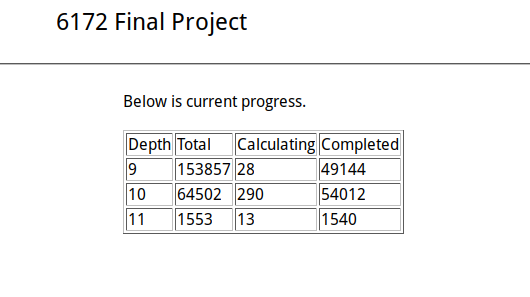
\includegraphics[scale=0.5]{screenshot1.png}
	\end{frame}
	
	\begin{frame}
		\frametitle{Openbook Results}
		
		\begin{itemize}
		\item Original Version: \textcolor{fgreen}{50\%} winrate against ReferencePlus.\pause
		\item Openbook VS Original: \textcolor{fgreen}{61\%} winrate.\pause
		\item However..\pause
		\item Openbook VS ReferencePlus: only \textcolor{dred}{45\%} winrate!
		\end{itemize}
	\end{frame}
	
	\begin{frame}
		\frametitle{Openbook Results}
		
		What might have happened?\pause
		
		\begin{itemize}
		\item[*] The opening patterns of ReferencePlus are not captured in the data 
		(at the time we capture data ReferencePlus is still not available).\pause
		\item[*] A deeper search doesn't gaurenteed a better move, but just gives a good move with higher probability. 
		An unlucky bad move in the hotspot of openbook might actually degrade performance.\pause
		\end{itemize}
		
		Experiments shows \textcolor{fgreen}{both} explanations are correct.
	\end{frame}
	
	\begin{frame}
		\frametitle{Boosting Openbook}
		
		Addressing the first possibility:\pause
		
		\textcolor{fgreen}{Add the games played against ReferencePlus into Openbook!}\pause
		
		\begin{itemize}
		\item[*] Before Boosting: \textcolor{dred}{45\%} winrate.\pause
		\item[*] After Round 1 Boosting (1500 games): \textcolor{fgreen}{50\%} winrate.\pause
		\item[*] After Round 2 Boosting (1500 games): \textcolor{fgreen}{56\%} winrate.\pause
		\item[*] After Round 3 Boosting (1500 games): \textcolor{fgreen}{61\%} winrate.\pause
		\end{itemize}
		
		Steady increase in winrate!
	\end{frame}
	
	\begin{frame}
		\frametitle{Boosting Openbook}
		
		Addressing the second possibility:\pause
		
		The bot has a largely different winrate between moving first (\textcolor{dred}{30\%}) and moving second (\textcolor{fgreen}{60\%}).\pause
		
		\begin{itemize}
		\item[*] Might the opening move ``h4g5'' actually be a bad move?\pause
		\item[*] Rotate the King in the first move!\pause
		\item[*] Now the game is very similar to as if we were moving second.\pause
		\end{itemize}
		
		Amazing winrate increase: from \textcolor{dred}{45\%} to \textcolor{fgreen}{60\%}!\pause
		
		Together with boosted openbook: \textcolor{fgreen}{69\%} winrate against ReferencePlus!
	\end{frame}
	
	\begin{frame}
		\frametitle{Our Final Openbook}
		
		In the end, our openbook:\pause
		\begin{itemize}
		\item[*] Contains about \textcolor{fgreen}{200000} game states arose from \textcolor{fgreen}{140000} games.\pause
		\item[*] Almost always hits \textcolor{fgreen}{6} rounds.\pause
		\item[*] With high probability hits \textcolor{fgreen}{7} or \textcolor{fgreen}{8} rounds.\pause
		\item[*] Can sometime even reach \textcolor{fgreen}{10} rounds or more.
		\end{itemize}
	\end{frame}
	
	\begin{frame}
		\frametitle{Boosting Openbook}
		
		remember to add in final result against refplus..
	\end{frame}
	
	
	
		
\end{document}